\SourcePage{776}{779}
\section*{\S\,a. Hermite Polynomials}
\addcontentsline{toc}{section}{a. Hermite Polynomials}
\markright{\S\,a. Hermite Polynomials}
\setcounter{figure}{51}

The equation
\begin{equation}
 y''-2xy'+2ny=0
 \tag{a.1}
\end{equation}
belongs to a class of equations soluble by the \emph{Laplace
method}\footnote{See, for example, É.~Goursat, \emph{Course in Mathematical
Analysis}, vol.~II, Moscow: Gostekhizdat, 1933; V.~I.~Smirnov, \emph{Course of
Higher Mathematics}, vol.~III, part 2, Moscow: Nauka, 1974.}.

In general, the method applies to linear equations of the form
\[
 \sum_{m=0}^{n}(a_m+b_mx)\frac{d^my}{dx^m}=0,
\]
whose coefficients are at most linear in $x$. Its procedure is as follows.
Form the polynomials
\[
 P(t)=\sum_{m=0}^{n}a_mt^m,\hspace{2em}
 Q(t)=\sum_{m=0}^{n}b_mt^m
\]
and from them construct
\[
 Z(t)=\frac1Q\exp\int\frac PQ\,dt,
\]
which is determined up to a constant factor. A solution of the equation can
then be written as the complex integral
\[
 y=\int_C Z(t)e^{xt}\,dt.
\]
The path $C$ is to be chosen so that this integral is finite and nonzero, and
the function
\[
 V=e^{xt}QZ
\]
must return to its initial value after $t$ has traversed the whole of $C$; the
contour may be either closed or open. For equation (a.1),
\[
 P=t^2+2n;\hspace{1.5em} Q=-2t,\hspace{1.5em}
 Z=-\frac1{2t^{n+1}}e^{-t^2/4},\hspace{1.5em}
 V=\frac1{t^n}e^{xt-t^2/4},
\]

\SourcePage{777}{780}
and hence its solution takes the form
\begin{equation}
 y=\int\exp\left(xt-\frac{t^2}{4}\right)\frac{dt}{t^{n+1}}.
 \tag{a.2}
\end{equation}

For physical applications it is sufficient to consider $n>-1/2$. At these
values either $C_1$ or $C_2$ in Fig.~52 may serve as the integration path. The
required conditions are satisfied because $V$ vanishes at their endpoints,
$t=+\infty$ or $t=-\infty$\footnote{These paths cannot be used for negative
integral $n$, since the integral (a.2) along either path would then vanish
identically.}.

We shall determine the values of $n$ for which (a.1) has a solution that is
finite at every finite $x$ and, as $x\to\pm\infty$, grows no faster than a
finite power of $x$. Begin with nonintegral $n$. Integration in (a.2) along
$C_1$ and $C_2$ gives two independent solutions. Transform the $C_1$ integral
by introducing $u$ through $t=2(x-u)$. On omitting a constant factor, the
result is
\begin{equation}
 y=e^{x^2}\int_{C'_1}\frac{e^{-u^2}}{(u-x)^{n+1}}\,du,
 \tag{a.3}
\end{equation}
where $C'_1$ is the contour in the complex $u$ plane shown in Fig.~53.

\begin{figure}[ht]
\centering
\begin{minipage}{.44\linewidth}\centering
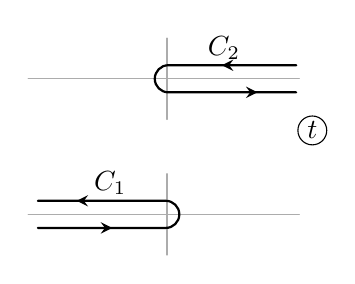
\begin{tikzpicture}[x=.82cm,y=.82cm,>=stealth,line cap=round,line join=round]
  \draw[gray!65,thin] (-2.15,1.05)--(2.05,1.05);
  \draw[gray!65,thin] (0,0.42)--(0,1.68);
  \draw[thick] (2.00,1.26)--(0.02,1.26)
    arc[start angle=90,end angle=270,radius=.21]--(2.00,.84);
  \draw[->,thick] (1.45,1.26)--(.85,1.26);
  \draw[->,thick] (.78,.84)--(1.40,.84);
  \node at (.88,1.52) {$C_2$};
  \draw[gray!65,thin] (-2.15,-1.05)--(2.05,-1.05);
  \draw[gray!65,thin] (0,-1.68)--(0,-.42);
  \draw[thick] (-2.00,-.84)--(-.02,-.84)
    arc[start angle=90,end angle=-90,radius=.21]--(-2.00,-1.26);
  \draw[->,thick] (-.78,-.84)--(-1.40,-.84);
  \draw[->,thick] (-1.45,-1.26)--(-.85,-1.26);
  \node at (-.88,-.56) {$C_1$};
  \node[circle,draw,inner sep=1.2pt] at (2.25,.25) {$t$};
\end{tikzpicture}
\caption{ }\label{fig:52}
\end{minipage}\hfill
\begin{minipage}{.44\linewidth}\centering
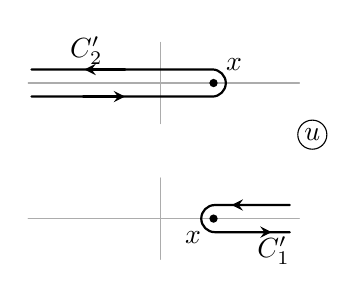
\begin{tikzpicture}[x=.82cm,y=.82cm,>=stealth,line cap=round,line join=round]
  \draw[gray!65,thin] (-2.05,1.05)--(2.15,1.05);
  \draw[gray!65,thin] (0,0.42)--(0,1.68);
  \fill (.82,1.05) circle (1.5pt);
  \draw[thick] (-2.00,1.26)--(.80,1.26)
    arc[start angle=90,end angle=-90,radius=.21]--(-2.00,.84);
  \draw[->,thick] (-.55,1.26)--(-1.18,1.26);
  \draw[->,thick] (-1.20,.84)--(-.55,.84);
  \node at (-1.15,1.55) {$C'_2$};
  \node[above right=1pt] at (.82,1.05) {$x$};
  \draw[gray!65,thin] (-2.05,-1.05)--(2.15,-1.05);
  \draw[gray!65,thin] (0,-1.68)--(0,-.42);
  \fill (.82,-1.05) circle (1.5pt);
  \draw[thick] (2.00,-.84)--(.84,-.84)
    arc[start angle=90,end angle=270,radius=.21]--(2.00,-1.26);
  \draw[->,thick] (1.72,-.84)--(1.10,-.84);
  \draw[->,thick] (1.08,-1.26)--(1.72,-1.26);
  \node at (1.75,-1.55) {$C'_1$};
  \node[below left=1pt] at (.82,-1.05) {$x$};
  \node[circle,draw,inner sep=1.2pt] at (2.35,.25) {$u$};
\end{tikzpicture}
\caption{ }\label{fig:53}
\end{minipage}
\end{figure}

As $x\to+\infty$, the whole contour $C'_1$ recedes to infinity, and the
integral in (a.3) tends to zero as $e^{-x^2}$. For $x\to-\infty$, however, the
integration path extends along the entire real axis and the integral in (a.3)
does not decrease exponentially; the leading growth of $y(x)$ is therefore
$e^{x^2}$. In the same way, one readily verifies that the integral (a.2) over
$C_2$ diverges exponentially as $x\to\infty$.

When $n$ is a nonnegative integer, the integrals over the straight parts of
the path cancel pairwise. Both versions of (a.3), over $C'_1$ and $C'_2$, then
reduce to an integral over a closed contour surrounding\SourcePage{778}{781}
the point $u=x$. We thus obtain the solution
\[
 y(x)=e^{x^2}\oint\frac{e^{-u^2}}{(u-x)^{n+1}}\,du,
\]
which has the required properties. By Cauchy's familiar formula for the
derivatives of an analytic function,
\[
 f^{(n)}(x)=\frac{n!}{2\pi i}\oint\frac{f(t)}{(t-x)^{n+1}}\,dt,
\]
this solution, apart from a constant factor, is the \emph{Hermite polynomial}
\begin{equation}
 H_n(x)=(-1)^ne^{x^2}\frac{d^n}{dx^n}e^{-x^2}.
 \tag{a.4}
\end{equation}

Expanded and ordered by descending powers of $x$, $H_n$ is
\begin{equation}
 H_n(x)=(2x)^n-\frac{n(n-1)}{1}(2x)^{n-2}
 +\frac{n(n-1)(n-2)(n-3)}{1\cdot2}(2x)^{n-4}-\ldots
 \tag{a.5}
\end{equation}
It contains only powers of $x$ having the same parity as $n$. The first few
Hermite polynomials are
\begin{equation}
 \begin{gathered}
 H_0=1,\hspace{1.25em} H_1=2x,\hspace{1.25em}
 H_2=4x^2-2,\hspace{1.25em} H_3=8x^3-12x,\\
 H_4=16x^4-48x^2+12.
 \end{gathered}
 \tag{a.6}
\end{equation}

To evaluate the normalization integral, substitute the expression (a.4) for
$e^{-x^2}H_n$ and integrate by parts $n$ times:
\[
 \int_{-\infty}^{+\infty}e^{-x^2}H_n^2(x)\,dx
 =\int_{-\infty}^{+\infty}(-1)^nH_n(x)
 \frac{d^n}{dx^n}e^{-x^2}\,dx
 =\int_{-\infty}^{+\infty}e^{-x^2}\frac{d^nH_n}{dx^n}\,dx.
\]
But $d^nH_n/dx^n$ is the constant $2^nn!$, and consequently
\begin{equation}
 \int_{-\infty}^{+\infty}e^{-x^2}H_n^2(x)\,dx=2^nn!\sqrt\pi.
 \tag{a.7}
\end{equation}
